\chapter{Simplicial Complexes and Homology}
\graphicspath{ {/home/tomasp/Dokumenty/Master_Thesis/figures/} }
%% Definitions, notations, remarks and examples
\theoremstyle{definition}
\newtheorem{definition}{Definition}[section]
\newtheorem{theorem}{Theorem}[section]
\newtheorem{lemma}{Lemma}[section]
\newtheorem{corollary}{Corollary}[section]
\newtheorem{example}{Example}[section]
\newtheorem*{remark}{Remark}

The goal of this and the following chapters is to establish and set up the pipeline for extracting the algebraic invariants of our data. Usually, we can only work with sampled and discrete data coming from some set of measurements. As such, we can't directly use methods of algebraic topology, since we won't typically be working with discrete topological spaces and to properly use these methods, we would need an uncountable amount of data; something that isn't feasible from a computational point of view.
\par
This forces us to use different methods to somehow approximate and recover the topology of the ambient space given only a finite set of points. Secondly, we also need to consider the \textit{scale} of the data -- some interesting properties may be more apparent only after we ``zoom'' in closely on them, some may not become apparent at all. All in all, we will construct the following pipeline:

\begin{center}
\smartdiagram[sequence diagram]{
  Discrete data, Simplicial complex, Algebraic invariants}
\end{center}

and repeat this step for all scales at once, effectively measuring the evolution of the algebraic invariants through the changes in the feature scale.

\section{Simplicial complexes}
\begin{definition}[Simplex]
For $k \geq 0$, a $k$-simplex $\sigma$ of dimension $k$ in a Euclidean space $\mathbb{R}^{n}$ is the convex hull of a set $P$ of $(k+1)$ affinely independent points in $\mathbb{R}^{n}$. For $0 \leq m \leq k$, an $m$-face of $\sigma$ is an $m$-simplex that is the convex hull of a nonempty subset of $P$. A \textit{proper face} of $\sigma$ is a simplex that is the convex hull of a proper subset of $P$ (any face except $\sigma$). $(k-1)$ faces of $\sigma$ are called \textit{facets} of $\sigma$.
\end{definition}

Typically, we refer to a $0$-simplex as a \textit{vertex}, a $1$-simplex as an \textit{edge}, a $2$-simplex as a \textit{triangle} and so on. An illustration of those can be seen in \ref{fig:simplex_1}.

\begin{figure}[h!]
  \centering
  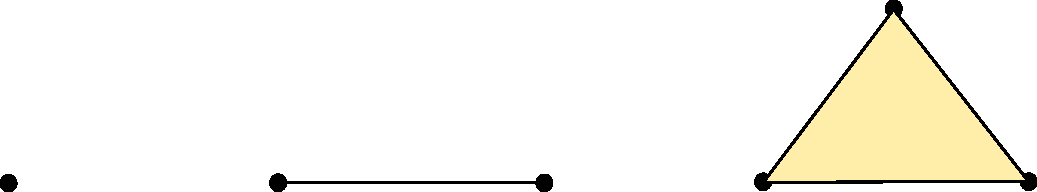
\includegraphics[width=10cm, height=2cm]{simplex_1.pdf}
  \caption{From the left: a $0$-simplex, a $1$-simplex and a $2$-simplex}
  \label{fig:simplex_1}
\end{figure}

\begin{definition}[Geometric simplicial complex]
  A \textit{geometric simplicial complex} $K$ is a set with finitely many simplices that satisfy the following:
  \begin{itemize}
    \item $K$ contains every face of each simplex in $K$.
    \item For any two simplices $\sigma, \tau \in K$, their intersection $\sigma \cap \tau$ is either empty or a face or both $\sigma$ and $\tau$.
  \end{itemize}
\end{definition}

This is also known as a \textit{triangulation}, where the \textit{dimension} $k$ of $K$ is the maximum dimension of any simplex in $K$. The two definitions above are highly geometric and easy to visualize and imagine. The next definition is more technical and abstract but nonetheless important.

\begin{definition}[Abstract simplex]
  A collection $K$ of non-empty subsets of a given set $V(K)$ is an \textit{abstract simplicial complex}, if every element $\sigma \in K$ has all of its non-empty subsets $\sigma' \subseteq \sigma$ also in $K$. Each element $\sigma$ with a cardinality $|\sigma| = k+1$ is called a $k$-simplex and each of its subsets $\sigma' \subseteq \sigma$ with $|\sigma'|=k'+1$ is called a $k'$-face. Finally, a $(k-1)$-face of a $k$-simplex is called its \textit{facet}.
\end{definition}

\begin{remark}
One could also dually define a $k$-coface, cofacet and its codimension but it's not terribly important.
\end{remark}

\begin{figure}[h!]
  \centering
  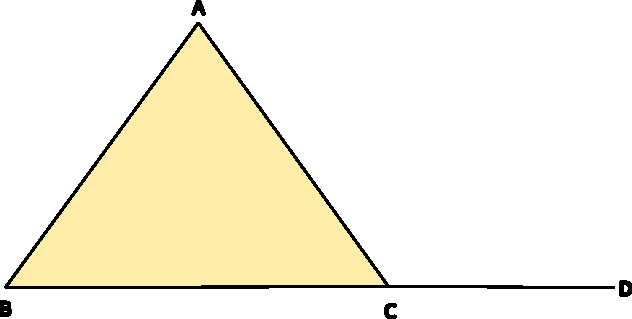
\includegraphics[width=8cm, height=4cm]{simplex_2.pdf}
  \caption{A simplicial complex with 4 vertices, 4 edges and 1 triangle.}
  \label{fig:simplex_2}
\end{figure}

A geometric simplicial complex $K$ in $\mathbb{R}^{n}$ is called a \textit{geometric realization} of an abstract simplicial complex $K'$, if and only if there is an embedding $e: V(K') \to \mathbb{R}^{n}$, that takes every $k$-simplex $\{v_{0}, \ldots, v_{k}\}$ in $K'$ to a $k$-simplex in $K$ that is the convex hull of $e(v_{0}), \ldots, e(v_{k})$. An example is shown in \ref{fig:simplex_2} as this is the geometric realization of the abstract complex with vertices $A,B,C,D,$ edges $\{A,B\}, \{A,C\}, \{B,C\}, \{C,D\}$ and 1 triangle $\{A,B,C\}$.

\begin{definition}[Underlying space]
  The \textit{underlying space} of an abstract simplicial complex $K$, denoted by $|K|$, is the pointwise union of its simplices in its geometrical realization, i.e., $|K| = \bigcup_{\sigma \in K}|\sigma|$, where $|\sigma|$ is the restriction of this realization on $\sigma$. If $K$ is geometric, then its geometric realization can be taken as itself.
\end{definition}

Unless it is considered necessary, we won't be making the distinction between the two due to this equivalence between geometric and abstract simplicial complexes.

\begin{definition}[$k$-skeleton]
  For any $k \geq 0$, the $k$-skeleton of a simplicial $K$ complex, denoted by $K^{k}$, is the subcomplex formed by all simplices of dimension at most $k$.
\end{definition}
Given this, in \ref{fig:simplex_2}, the $1$-skeleton consists of the vertices $A,B,C,D$ and the edges joining those.

\section{Nerves, Čech and Rips complexes}
Given any open cover of a topological space, we are able to construct a simplicial complex on top of it. As we'll see, there isn't only one kind of complex we can build, depending on the properties we're looking for and its size, which has to be considered whenever we talk about any software implementation of the algorithms.

\begin{definition}[Nerve]
  Given a finite collection of sets $\mathfrak{U} = \{U_{\alpha}\}_{\alpha \in A}$, we define the \textit{nerve} of the set $\mathfrak{U}$ to be the simplicial complex $N(\mathfrak{U})$, whose vertex set is the index set $A$, and where a subset $\{\alpha_{0}, \ldots, \alpha_{k}\} \subseteq A$ spans a $k$-simplex in $N(\mathfrak{U})$ if and only if $U_{\alpha_{0}} \cap \ldots \cap U_{\alpha_{k}} \ne \emptyset$.
\end{definition}

\begin{figure}[h!]
  \centering
  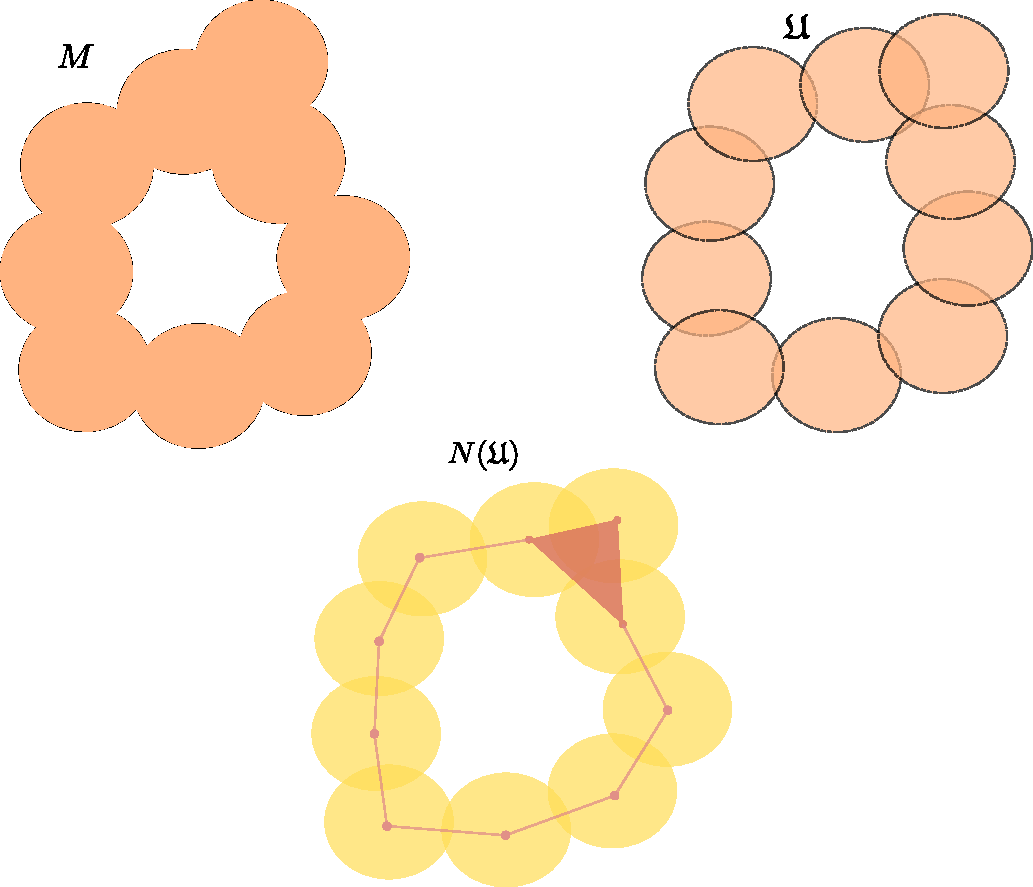
\includegraphics[width=10cm, height=8cm]{nerve_1.pdf}
  \caption{An example of a space $M$, its open cover $\mathfrak{U}$ and its nerve $N(\mathfrak{U})$.}
  \label{fig:nerve_1}
\end{figure}

The following important theorem about nerves tells us when are the nerves ``equivalent'' to the original space. There are various formulation of this statement but since we are working primarily with finite metric spaces, we'll adopt the appropriate version for it.

\begin{theorem}[Nerve theorem]
  Given a finite cover $\mathfrak{U}$ (open or closed) of a metric space $M$, the underlying space $|N(\mathfrak{U})|$ is homotopy equivalent to $M$, if every non-empty intersection $\cap_{i=0}^{k}U_{\alpha_{i}}$ of cover elements is homotopy equivalent to a point, i.e., contractible.
\label{theorem:Nerve theorem}
\end{theorem}

For those interested in a proof of this statement, see \cite{Borsuk1948OnTI} for example. From this we can see, that the nerve is homotopy equivalent to $M$ in \ref{fig:nerve_1}. Now we can finally present the first construction of an abstract simplicial complex using the concept of a nerve, given a finite subset $P$ of a metric space $(M,d)$.

\begin{definition}[Čech complex]
  Let $(M,d)$ be a metric space and $P$ a finite subset of it. Given a real $r > 0$, the Čech complex $\mathbb{C}^{r}(P)$ is defined to be the nerve of the set $\{B(p_{i},r)\}$, where
  \begin{equation*}
    B(p_{i},r) = \{x \in M \: \vert \: d(p_{i},x) \leq r \}.
  \end{equation*}
\end{definition}

One can easily deduce that if $M$ happens to be a Euclidean metric space, according to Theorem~\ref{theorem:Nerve theorem}, the Čech complex will be homotopy equivalent to the space of union of the balls. The Čech complex has nice theoretical properties, but the one predominantly implemented in most software packages is the Vietoris-Rips complex bellow.

\begin{definition}[Vietoris-Rips complex]
  Let $(P,d)$ be a finite metric space. Given a real $r>0$, the Vietoris-Rips (VR for short) complex is the abstract simplicial complex $\mathbb{VR}^{r}(P)$, where a simplex $\sigma \in \mathbb{VR}^{r}(P)$, if and only if $d(p,q) \leq 2r$ for every pair of vertices of $\sigma$.
\end{definition}

\begin{figure}[h!]
  \centering
  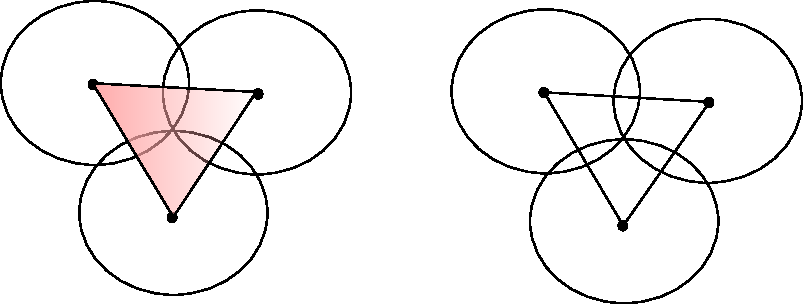
\includegraphics[width=8cm, height=4cm]{CechVR.pdf}
  \caption{On the left, the VR complex of three pairwise intersecting triangles. On the right, the corresponding Čech complex.}
  \label{fig:CechVR}
\end{figure}

A simple example, where we can see the difference between the Čech and VR complex can be seen on \ref{fig:CechVR}. For an interactive visualization of the two, the reader may want to access the following sites - \cite{smajhiVietorisx2013RipsComplex} and \cite{saulnechComplex}. With the movement of the sliders there, the reader is introduced to another important concept that we will make use of - changing the radius $r$ and constructing a growing sequence of either Čech or VR complexes.

Nevertheless, we don't have to worry too much about the differences between the two, given the following result.

\begin{theorem}
  Let $P$ be a finite subset of a metric space $(M,d)$. Then
  \begin{equation}
    \mathbb{C}^{r}(P) \subseteq \mathbb{V}^{r}(P) \subseteq \mathbb{C}^{2r}(P).
  \end{equation}
\end{theorem}

\section{Sparse complexes}

While the VR complex is the one you will usually encounter in most talks about TDA, it has a size problem. More often than not, both the Čech and VR complexes grow too large, even in low dimensions. A VR complex constructed out of a few thousand points can easily have millions of triangles. A short example of this behaviour can be seen in \ref{fig:sizeofVR}. As such, sometimes it is computationally less expensive to use more sparse alternatives instead. \footnote{Technically, the graph is based on the Rips filtration, a term we'll see in the future although it doesn't change the point presented here.}

\begin{figure}[h!]
  \centering
  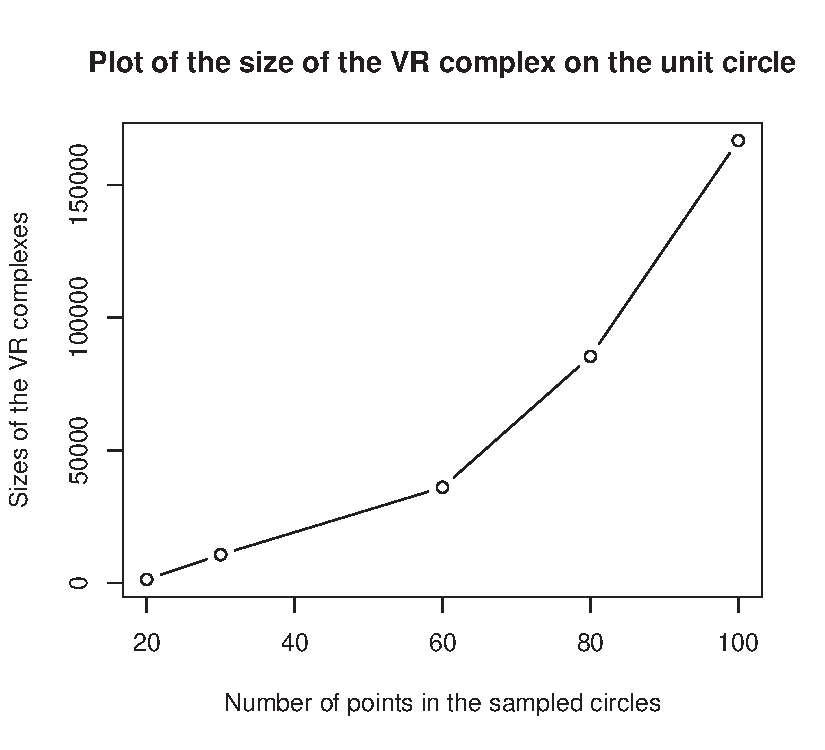
\includegraphics[width=8cm, height=8cm]{sizeofVR.pdf}
  \caption{An illustration of the growth of the VR complex when we increase the number of sampled points.}
  \label{fig:sizeofVR}
\end{figure}

\subsection{Delaunay complex}

This complex is usually used in various applications, such as mesh generation or 3D triangulation (for example, see \href{https://doc.cgal.org/latest/Manual/packages.html#PartTriangulationsAndDelaunayTriangulations}{the following}). However, it remains computationally expensive in dimensions greater than 3, and other complexes are preferred instead.

\begin{definition}[Delaunay complex]
Let $P$ be a finite point set in $R^{n}$. A $k$-simplex $\sigma$ is called \textit{Delaunay}, if its vertices are in P and there is an open $n$-ball whose boundary contains the boundary of this ball. A \textit{Delaunay complex} of $P$, denoted by Del $P$, is the simplicial complex with vertices in $P$, in which every simplex is Delaunay and $\vert$ Del $P \vert$ coincides with the convex hull of $P$.
\end{definition}

The Delaunay complex is dual to another construction that you may or may not encounter in the wild - the Voronoi diagram.

\begin{definition}[Voronoi diagram]
  Given a finite point set $P \subset \mathbb{R}^{n}$ in generic position, the Voronoi diagram Vor($P$) of $P$ is the tessellation of the embedding space $\mathbb{R}^{n}$ into convex cells $V_{p}$ for every $p \in P$ where
  \begin{equation*}
    V_{p} = \{x \in \mathbb{R}^{n} \: \vert \: d(x,p) \leq d(x,q), \forall q \in P\}.
  \end{equation*}
  Additionally, a $k$-face of Vor($P$) is the intersection of $(d-k+1)$ Voronoi cells.
\end{definition}

The duality between a Delaunay complex and Voronoi diagram is better expressed through this little theorem.
\begin{theorem}
  For $P \in \subset \mathbb{R}^{n}$, Del($P$) is the nerve of the set of Voronoi cells $\{V_{p}\}_{p \in P}$, which is a closed cover of $\mathbb{R}^{n}$.
\end{theorem}
More specifically, a Delaunay $k$-simplex in Del($P$) is dual to a Voronoi $(d-k)$-face in Vor($P$).

The reasons why Delaunay complexes are popular in dimensions $<3$ are the following
\begin{theorem}
  A triangulation of a point set $P \subset \mathbb{R}^{n}$ is a geometric simplicial complex whose vertex set is $P$ and whose simplices tessellate the convex hull of $P$. Among all triangulations of a point set $P \subset \mathbb{R}^{n}$, Del($P$) achieves the following:
  \begin{enumerate}
    \item In $\mathbb{R}^{2}$, Del($P$) maximizes the minimum angle of triangles in the complex.
    \item In $\mathbb{R}^{2}$, Del($P$) minimizes the largest circumcircle for triangles in the complex.
    \item For a simplex in Del($P$), let its min-ball be the smallest ball that contains the simplex in it. In all dimensions, Del($P$) minimizes the largest min-ball.
  \end{enumerate}
\end{theorem}
Unfortunately, the size of a Delaunay complex is $O(n^{\lceil d/2 \rceil})$, with the same cost in computation (see \cite{chazelle1993optimal}).

\subsection{Alpha complex}
Alpha complexes are parametrized subcomplexes of the Delaunay complex by some real $\alpha \geq 0$.
